% figures/steering_heatmap.tex -- Steering results summary
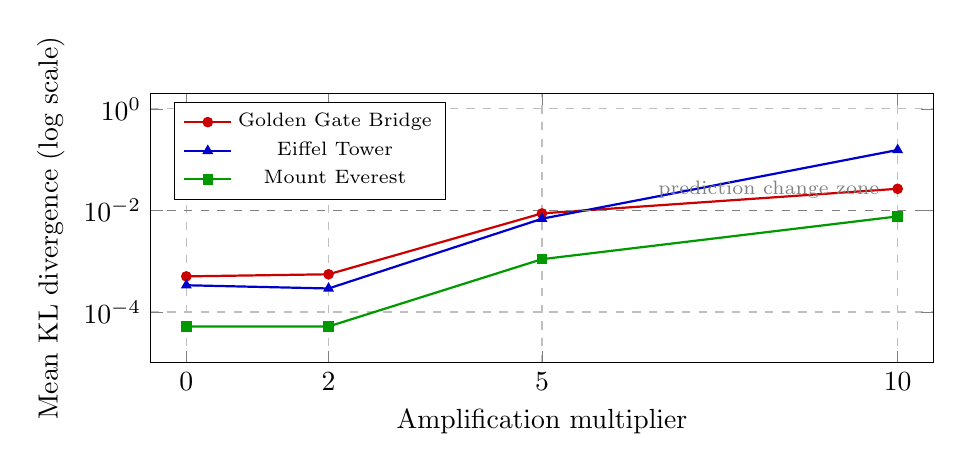
\begin{tikzpicture}
\begin{axis}[
    width=0.95\columnwidth,
    height=5cm,
    xlabel={Amplification multiplier},
    ylabel={Mean KL divergence (log scale)},
    xmin=-0.5, xmax=10.5,
    xtick={0, 2, 5, 10},
    ymode=log,
    ymin=1e-5, ymax=2,
    legend pos=north west,
    legend style={font=\scriptsize},
    grid=major,
    grid style=dashed,
]

% Golden Gate Bridge
\addplot[color=red!80!black, thick, mark=*, mark size=1.5pt] coordinates {
    (0, 0.000504) (2, 0.000554) (5, 0.008766) (10, 0.026760)
};
\addlegendentry{Golden Gate Bridge}

% Eiffel Tower
\addplot[color=blue!80!black, thick, mark=triangle*, mark size=1.5pt] coordinates {
    (0, 0.000337) (2, 0.000291) (5, 0.006882) (10, 0.155421)
};
\addlegendentry{Eiffel Tower}

% Mount Everest
\addplot[color=green!60!black, thick, mark=square*, mark size=1.5pt] coordinates {
    (0, 0.000052) (2, 0.000052) (5, 0.001099) (10, 0.007649)
};
\addlegendentry{Mount Everest}

% Annotation for prediction change threshold
\draw[dashed, gray, thin] (axis cs:-0.5, 0.01) -- (axis cs:10.5, 0.01);
\node[font=\scriptsize, gray, anchor=south west] at (axis cs:6.5, 0.011)
    {prediction change zone};

\end{axis}
\end{tikzpicture}
